\chapter{Module Role and Scope}

The Coffee Chain ERP system plays a vital role in consolidating operations while maintaining clear boundaries for functionality. This chapter defines both the role and scope of the system.

\section*{Role of the ERP Module}
The primary role of the Coffee Chain ERP is to act as an integrative backbone for coffee chain operations:
\begin{itemize}
    \item \textbf{Unification:} Combines outlet, menu, sales, and CRM functions into one system.  
    \item \textbf{Consistency:} Ensures standardized processes across all outlets.  
    \item \textbf{Insight:} Provides managers with real-time and historical data for decision-making.  
    \item \textbf{Scalability:} Prepares the system for future growth, such as adding loyalty features or advanced analytics.  
\end{itemize}

\section*{Scope of the Coffee Chain ERP}
The scope defines current inclusions and exclusions:
\begin{itemize}
    \item Covers active coffee outlets and their daily operations.  
    \item Includes menu item management, pricing, and categorization.  
    \item Captures all sales orders and integrates them with reporting dashboards.  
    \item Synchronizes CRM data with sales transactions for lead tracking.  
    \item Excludes loyalty and reward systems, outlet capacity tracking, and HR functions.  
\end{itemize}

\section*{Stakeholders and KPIs}
Different stakeholders rely on the system for performance insights:
\begin{itemize}
    \item \textbf{Outlet Managers:} Track efficiency and revenue.  
          \textit{KPIs: daily revenue, sales per product.}
    \item \textbf{Regional Managers:} Compare multiple outlets.  
          \textit{KPIs: average outlet growth, variance analysis.}
    \item \textbf{Employees:} Maintain data quality.  
          \textit{KPIs: error rate in transactions, product data accuracy.}
    \item \textbf{Top Management:} Align operations with strategy.  
          \textit{KPIs: conversion rates, long-term revenue growth.}
\end{itemize}

\section*{Context Diagram (C1)}
\begin{figure}[H]
\centering
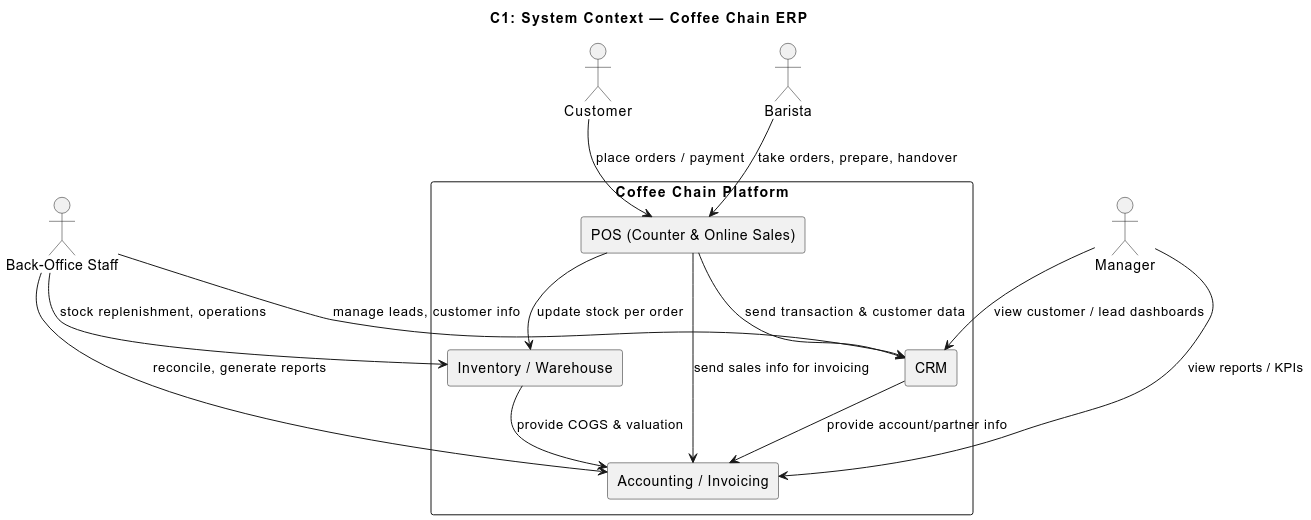
\includegraphics[width=0.9\textwidth,keepaspectratio]{diagrams/context.png}
\caption{C1-Level Context Diagram of Coffee Chain ERP}
\end{figure}

\section*{Insights}
\begin{itemize}
    \item The module consolidates roles and responsibilities into one backbone.  
    \item Defined boundaries prevent scope creep while leaving room for growth.  
    \item KPIs provide measurable indicators of performance at each level.  
\end{itemize}
